\subsection{Diseño Módulo 3}
En esta sección se presenta el diseño del módulo 3 correspondiente a la base de datos, 
cuya función principal consiste en la
gestión y almacenamiento de los datos recopilados por los sensores conectados a los
microcontroladores instalados en los frascos del módulo 1.
\newline
Por lo que para llevar a cabo dicho diseño, se llevó a cabo un proceso sistemático
de normalización de datos en cada una de las tablas que componen la base de datos 
, con el fin de optimizar el almacenamiento y la
eficiencia en las consultas, además de reducir la redundancia y mejorar la integridad de
los datos. 
\newline
El diseño parte del modelo entidad-relación (ER) mostrado en la \cref{fig:ModeloER}, 
en el cual se identifican claramente las entidades principales y sus interrelaciones. 
En dicho modelo, el módulo 1 se encarga de la adquisición de los datos 
provenientes de los sensores; por su parte, 
el módulo 2 realiza el análisis de los datos recopilados; 
finalmente, los usuarios finales quienes interactúan con el sistema mediante una interfaz
web pueden pertenecer a distintas categorías, destacando los productores 
iniciales o los productores raíz derivados de estos últimos.
\newline
Por ende, a primera instancia no va a estar normalizado, ya que se busca tener una visión
general de las tablas y sus relaciones, para posteriormente llevar a cabo de manera progresiva, la
normalización de los datos hasta alcanzar la tercera forma normal.
\newline
Asimismo, se elabora un diagrama de relación que representa las entidades,
atributos y relaciones entre las tablas de la base de datos, facilitando la comprensión
de la estructura y las interacciones entre los diferentes componentes del sistema..


\begin{figure}[htb]
\centering
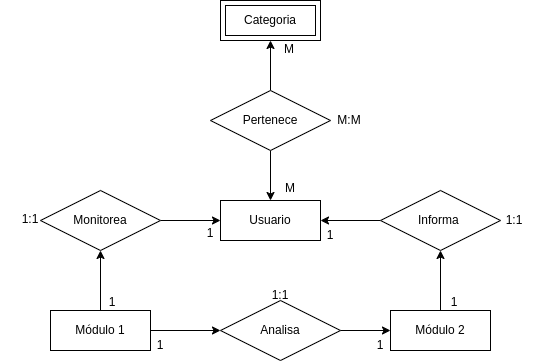
\includegraphics[width=0.9\textwidth]{./UML/Modulo3/modeloER.drawio.png}
\caption{Moelo Entidad-Relación}
\label{fig:ModeloER}
\end{figure} 

\subsubsection{Normalización de datos}
Por lo tanto para llevar a cabo la normalización de los datos, 
se ha tomado como referencia la tablas previamente definidas en la sección 
, con el fin de normalizar los datos 
correspondientes a las tres primeras formas normales (1NF, 2NF y 3NF).

A continuación, se presenta la tabla original y su descripción, seguida de la tabla
normalizada hasta la forma correspondientes de cada una de las tres primeras formas normales (1NF, 2NF y 3NF).

Apartir de la \cref{tab:Usuario} siendo esta la tabla
central, se procede a realizar la normalización de los datos.
Obteniendo la tabla  las siguientes tablas normalizadas:
En la  \cref{tab:Usuario} se definen los atributos del usuario, incluyendo
información personal y de contacto, así como detalles relacionados con el proceso y
nodo asociado al usuario.
En la \cref{tab:Categoría} se define la categoría del usuario, vinculada a su
identificador único.Siendo esta la relación con otros usuarios productores.
En la \cref{tab:Dirección} se definen los atributos relacionados con la dirección
del usuario, incluyendo ciudad, colonia, municipio, código postal, calle y número.
En la \cref{tab:Proceso} se definen los atributos del proceso asociado al usuario,
incluyendo eficiencia, estado y nivel del proceso, siendo esta tabla relacionada con
el módulo 2.


\begin{table}[htbp]
    \centering
    \caption{Atribudos del Usuario} % Título Corregido (Ver Sección 2)
    \label{tab:Usuario}
    \footnotesize % Reducimos el tamaño de la fuente para ayudar al ajuste

    % Ajuste de Anchos de Columna (el ancho total debe sumar < 16cm)
    \begin{tabular}{|>{\raggedright\arraybackslash}p{2.5cm}|c|}
        \hline
        \textbf{Atributo}       & \textbf{Tipo de Dato}  \\ \hline
        ID del usuario          & varchar(20)  \\ \hline
        Categoría del usuario   & varchar(15) \\ \hline
        ID del proceso          & INT          \\ \hline
        ID del nodo             & VARCHAR(20)  \\ \hline
        Eficiencia              & FLOAT        \\ \hline
        Nombre                  & varchar(20)  \\ \hline 
        Primer Apellido         & varchar(20)  \\ \hline
        Segundo Apellido        & varchar(20)  \\ \hline
        Género                  & varchar(15)  \\ \hline
        Ciudad                  & varchar(20)  \\ \hline
        Colonia                 & varchar(20)  \\ \hline
        Municipio               & varchar(20)  \\ \hline
        C.P.                      & varchar(10) \\ \hline
        Calle                   & varchar(30)  \\ \hline
        Número                  & INT          \\ \hline
        Teléfono                & INT          \\ \hline
        Correo                  & varchar(20)  \\ \hline
        
    \end{tabular}
\end{table}


\begin{table}[htbp]
    \centering
    \caption{Usuario} % Título Corregido (Ver Sección 2)
    \label{tab:Usuario}
    \footnotesize % Reducimos el tamaño de la fuente para ayudar al ajuste

    % Ajuste de Anchos de Columna (el ancho total debe sumar < 16cm)
    \begin{tabular}{|>{\raggedright\arraybackslash}p{2.5cm}|c|}
        \hline
        \textbf{Atributo}       & \textbf{Tipo de Dato}  \\ \hline
        \textbf{PK} ID del usuario & varchar(20)  \\ \hline
        FK ID del proceso          & INT          \\ \hline
        FK ID del nodo             & VARCHAR(20)  \\ \hline
        FK Ciudad                  & varchar(20)  \\ \hline
        Nombre                  & varchar(20)  \\ \hline 
        Primer Apellido         & varchar(20)  \\ \hline
        Segundo Apellido        & varchar(20)  \\ \hline
        Género                  & varchar(15)  \\ \hline
        Teléfono                & INT          \\ \hline
        Correo                  & varchar(20)  \\ \hline
        
    \end{tabular}
\end{table}

\begin{table}[htbp]
    \centering
    \caption{Categoría} % Título Corregido (Ver Sección 2)
    \label{tab:Categoría}
    \footnotesize % Reducimos el tamaño de la fuente para ayudar al ajuste

    % Ajuste de Anchos de Columna (el ancho total debe sumar < 16cm)
    \begin{tabular}{|>{\raggedright\arraybackslash}p{2.5cm}|c|}
        \hline
        \textbf{Atributo}       & \textbf{Tipo de Dato}  \\ \hline
        Categoría del usuario   & varchar(15) \\ \hline
        Id del usuario          & varchar(20)  \\ \hline
    \end{tabular}
\end{table}


\begin{table}[htbp]
    \centering
    \caption{Dirección} % Título Corregido (Ver Sección 2)
    \label{tab:Dirección}
    \footnotesize % Reducimos el tamaño de la fuente para ayudar al ajuste

    % Ajuste de Anchos de Columna (el ancho total debe sumar < 16cm)
    \begin{tabular}{|>{\raggedright\arraybackslash}p{2.5cm}|c|}
        \hline
        \textbf{Atributo}       & \textbf{Tipo de Dato}  \\ \hline
        Ciudad                  & varchar(20)  \\ \hline
        Colonia                 & varchar(20)  \\ \hline
        Municipio               & varchar(20)  \\ \hline
        C.P.                      & varchar(10)  \\ \hline
        Calle                   & varchar(30)  \\ \hline
        Número                  & INT          \\ \hline  
    \end{tabular}
\end{table}

\begin{table}[htbp]
    \centering
    \caption{Proceso}% Título Corregido (Ver Sección 2)
    \label{tab:Proceso}
    \footnotesize % Reducimos el tamaño de la fuente para ayudar al ajuste

    % Ajuste de Anchos de Columna (el ancho total debe sumar < 16cm)
    \begin{tabular}{|>{\raggedright\arraybackslash}p{2.5cm}|c|}
        \hline
        \textbf{Atributo}       & \textbf{Tipo de Dato}  \\ \hline
        Id del proceso          & INT          \\ \hline
        Eficiencia              & FLOAT        \\ \hline
        Estado                  & varchar(20)  \\ \hline % Ajustado: Nombre no es Tinyint
        Nivel                   & varchar(20)  \\ \hline
    \end{tabular}
\end{table}



Asimismo se presenta la \cref{tab:lecturas_kefir} siendo esta la tabla
del módulo 1, de la cual al normalizarla se obtienen las siguientes tablas normalizadas:
En la \cref{tab:Nodo} se definen los atributos del nodo, incluyendo su identificador único y la
marca de tiempo de la lectura.
En la \cref{tab:alarma} se definen los atributos de la alarma, vinculada al nodo
correspondiente.
En la \cref{tab:sensado} se definen los atributos del sensado, incluyendo la marca de
tiempo y las lecturas de temperatura, pH y CO2


\begin{table}[htbp]
    \centering
    \caption{Atributos de los sensores}
    \label{tab:lecturas_kefir}
    \begin{tabular}{|>{\raggedright\arraybackslash}p{2.5cm}|c|}
                                 
        \hline
        \textbf{Atributo}         & \textbf{Tipo de dato}      \\ \hline
        ID del nodo               & VARCHAR(20)                 \\ \hline
        Timeset                   & TIMESTAMP                  \\ \hline
        ph                        & FLOAT                      \\ \hline
        $CO_{2}$                      & FLOAT                      \\ \hline
        temperatura               & FLOAT                      \\ \hline
        bandera\_alarma           & VARCHAR(20)                \\ \hline
    \end{tabular}
\end{table}

\begin{table}[htbp]
    \centering
    \caption{Nodo}
    \label{tab:Nodo}
    \small
   \begin{tabular}{|>{\raggedright\arraybackslash}p{2.5cm}|c|}
        \hline
        \textbf{Atributo}         & \textbf{Tipo de dato}      \\ \hline
        ID del nodo               & VARCHAR(20)                 \\ \hline
        Timeset                   & TIMESTAMP                  \\ \hline
    \end{tabular}
\end{table}


\begin{table}[htbp]
    \centering
    \caption{Alarma}
    \label{tab:alarma}
    \small
    \begin{tabular}{|>{\raggedright\arraybackslash}p{2.5cm}|c|}
        \hline
        \textbf{Atributo}         & \textbf{Tipo de dato}      \\ \hline
        ID del nodo               & VARCHAR(20)                 \\ \hline
        bandera de alarma           & VARCHAR(20)                \\ \hline
   \end{tabular}
\end{table}

\begin{table}[htbp]
    \centering
    \caption{Medición}
    \label{tab:sensado}
    \small
    \begin{tabular}{|>{\raggedright\arraybackslash}p{2.5cm}|c|}
        \hline
        \textbf{Atributo}         & \textbf{Tipo de dato}      \\ \hline
        Timeset                   & TIMESTAMP                  \\ \hline
        Temperatura               & FLOAT                      \\ \hline
        ph                        & FLOAT                      \\ \hline
        $CO_{2}$                  & FLOAT                      \\ \hline
   \end{tabular}
\end{table}

\begin{figure}[htb]
\centering
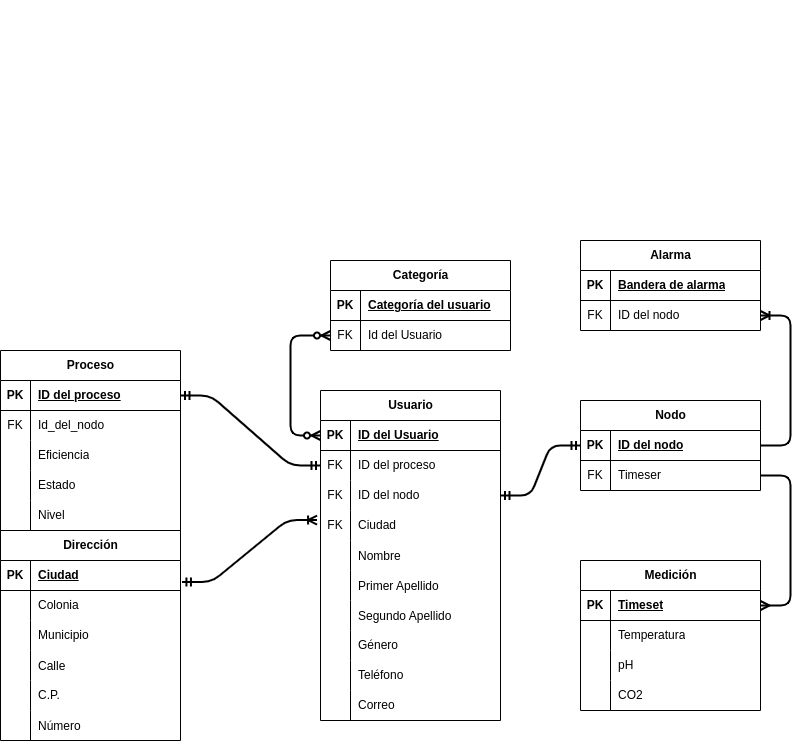
\includegraphics[width=0.9\textwidth]{./UML/Modulo3/diseno3.drawio.png}
\caption{Diagrama Relacional}
\label{fig:DiagramaR}
\end{figure} 
